\documentclass[a4paper]{article}

\usepackage[english]{babel}
\usepackage[utf8]{inputenc}
\usepackage{amsmath}
\usepackage{graphicx}
\usepackage[colorinlistoftodos]{todonotes}
\usepackage{listings}
\addtolength{\textwidth}{1in}
\addtolength{\oddsidemargin}{-.5in}

\title{System Validation 2016 \\ Homework Part 2 - Model Checking}

\author{Koen Mulder (s1757679) and Ruben van den Berg (s1354914)}

\date{\today}

\begin{document}
	\maketitle
	
	\begin{abstract}
		This homework assignment is done for the course System Validation. Here has been practiced with Model checking through Temporal Logic, NuSMV and SatAbs. In the first part formal requirements were generated for a water lock. In the second part an interlocking system for railway tracks is formalized with the help op NuSMV. Finally a simple array out-of-bounds violations are checked with SatAbs. 
	\end{abstract}
	
	\section{Lock Requirements}
	The first exercise relates to the lock specification exercise as given in the first exercise session of the course. Below all informal requirements are given and a JML or temporal logic specification to solve this. For each it is specified which solution is used behind the requirement itself.
	For the JML specifications the following variables are used:
	\begin{lstlisting}
float waterLevelLock;
float waterLevelRight;
float waterLevelLeft;
boolean rightDoorOpen;
boolean leftDoorOpen;
int shipsWaitingRight;
int shipsWaitingLeft;
int shipsInLock;
boolean shipBetweenDoors; // The ship being in an open door
	\end{lstlisting}
	For the Temporal Logic specifications the following variables are used:
	\begin{lstlisting}
left_door : {open, closed, opening, closing};
right_door : {open, closed, opening, closing};
audio_signal : {on, off};
boat_location : {left, right, entering_left, entering_right, in_lock};
	\end{lstlisting}
	\begin{itemize}
		\item There must be water within the lock (JML).
		\begin{lstlisting}
//@ invariant waterLevelLock > 0;
		\end{lstlisting}
		The water level within the lock is higher then 0 meters.
		
		\item The water in the lock should be at least 5 meters deep (JML).
		\begin{lstlisting}
//@ invariant waterLevelLock > 5;
		\end{lstlisting}
		The water level within the lock is higher then 5 meters.
		
		\item The gate should not open if the water level in the lock is lower than the water level on the other side(JML).
		\begin{lstlisting}
//@ requires waterLevelLock >= waterLevelRight;
void OpenRightDoor() {
}
//@ requires waterLevelLock >= waterLevelLeft;
void OpenLeftDoor() {
}
		\end{lstlisting}
		According to the specification the doors only open if the water level within the lock is equal or higher then the water level on the other side of the lock. However in our opinion it should only open when the water level is equal.
		
		\item There should be a boat inside before raising the water (JML).
		\begin{lstlisting}
//@ requires shipsInLock == 1;
void RaiseWater() {
}
		\end{lstlisting}
		It requires one ship within the lock to raise the water. However now a waiting boat on the higher side, needs to wait for another boat to come up before able to go down. It should also raise the water if there is a boat waiting.
		
		\item Only one door can be opened at a time (JML).
		\begin{lstlisting}
//@ requires !rightDoorOpen;
void OpenLeftDoor() {
}
//@ requires !leftDoorOpen;
void OpenRightDoor() {
}	
		\end{lstlisting}
		If the left door should open the right door can not be open and vice versa.
		
		\item Boats should be able to get to the other side of the lock (temporal).
		\begin{lstlisting}
LTLSPEC G((boat_location = left & X(boat_location = entering_left)) ->
F boat_location = right);
LTLSPEC G((boat_location = right & X(boat_location = entering_right)) ->
F boat_location = left);
		\end{lstlisting}
		If a boat has a location left or right and the next state is that he is entering (in this case you dismiss boats who are leaving the lock), he should finally arrive at the other side of the lock. 
		
		\item Boats can only pass one at a time(JML).
		\begin{lstlisting}
//@ invariant shipsInLock == 0 || shipsInLock == 1;
		\end{lstlisting}
		Within the lock there can be either 0 or 1 ships.
		
		\item There should be an audio signal whenever the gate opens or closes (temporal).
		\begin{lstlisting}
LTLSPEC G(left_door = opening -> X audio_signal = on);
LTLSPEC G(left_door = closing -> X audio_signal = on);
LTLSPEC G(right_door = opening -> X audio_signal = on);
LTLSPEC G(right_door = closing -> X audio_signal = on);
		\end{lstlisting}
		If a door is opening or closing the next state should be an audio signal turning on.
		
		\item When a boat has entered, the doors should close(temporal).
		\begin{lstlisting}
LTLSPEC G((boat_location = entering_left && X(boat_location = in_lock)) ->
F (left_door = closed & right_door = closed));
LTLSPEC G((boat_location = entering_right && X(boat_location = in_lock)) ->
F (left_door = closed & right_door = closed));
		\end{lstlisting}
		If a boat is entering and the next state is that he is in the lock (in this case you dismiss boats who are leaving the lock), both doors should close.
		
		\item The doors should not close when a boat goes in (JML).
		\begin{lstlisting}
//@ requires !shipBetweenDoors;
void CloseRightDoor() {
}
//@ requires !shipBetweenDoors;
void CloseLeftDoor() {
}
		\end{lstlisting}
		If a door needs to close it requires that there is not a boat between the doors.
	\end{itemize}
	
	\section{SMV and Temporal Logics}
	\begin{figure}[h]
		\centering
		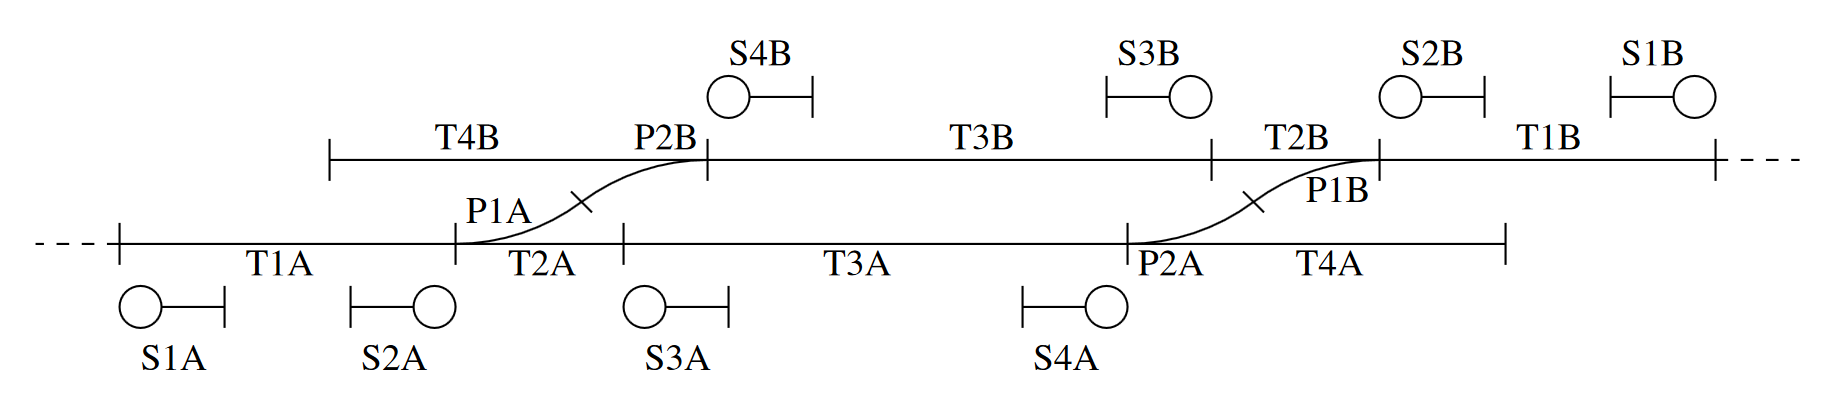
\includegraphics[width=\textwidth]{switches.PNG}
		\caption{The layout of the passing area.}
	\end{figure}
	
	\subsection{Properties}
	the properties we have written are visible in the \textit{\textbf{properties.smv}} file that comes with this report.
	During the creation of these properties we made multiple assumptions, these we will mention in this section.
	
	One of the assumptions we made was about the track parts \texttt{T4A} and \texttt{T4B}. According to the specifications it is allowed to move onto this piece of track as there is no mention otherwise, also according to the image there seems to be a relative big piece of track compared to the other switch tracks \texttt{T2A} and \texttt{T2B}. Based on this we made the assumption that the signals \texttt{S4A} and \texttt{S4B} can be green if they are locked straight. In this case a requirement similar to:
	\begin{lstlisting}
LTLSPEC G((T4A_occupied & P2A_locked_straight) -> S4A_red)
LTLSPEC G(((!P1B_locked_curved | T2B_occupied | T1B_occupied | T4A_occupied) 
& P2A_locked_curved) -> S4A_red)
LTLSPEC G((!P2A_locked_straight & !P2A_locked_curved) -> S4A_red)
	\end{lstlisting}
	Would be replaced with:
	\begin{lstlisting}
LTLSPEC G(((!P1B_locked_curved | T2B_occupied | T1B_occupied | T4A_occupied) 
& P2A_locked_curved) -> S4A_red)
LTLSPEC G(!P2A_locked_curved -> S4A_red)
	\end{lstlisting}
	
	A situation where we partly deviated from the specifications is in the case of \textit{\textbf{The points always follow the given commands}}. This partly has to do with our interpretation of the specification and with the functions of the system. In our interpretation we interpreted this requirement as when a goal is given it has to follow the order before having a new order. However this will not work in a situation with multiple trains. In some situations a certain order has priority over an other one. This is the case with 2 trains at \texttt{T1A} and \texttt{T3B}. In the example first a train would arrive at \texttt{T3B}, setting the goal of 2 points to curved. However then a train arrives at \texttt{T1A}, the goals of the points are set to straight while their never entered a locked curved position.
	Because of this situation we added this as an exception. The a goal curved can be replaced by a goal straight, as long as it will still eventually be locked curved. However depending on the interpretation of the informal requirements this still can be correct behavior.
	
	\subsection{Error case counter example}
	The error case is checked and generates multiple errors with counter examples. Here we describe one of the counterexamples for the following specification: 
	\begin{lstlisting}
G((T2A_occupied &  X T3A_occupied) -> F T4A_occupied)
	\end{lstlisting}
	Sign 1A is red while the points are moving to straight. As soon as they are locked straight the sign 1A goes to green and track 1A is occupied by a train. Sign 2A also goes to green. The train moves to track 2A and afterwards sign 2A goes to red. Then the train moves to track 3A, sign 3A goes to green and sign 1B goes to red. The points 1B and 2A are both locked straight. The points starting moving to curved. Then a train enters track 1B and sign 2B goes to red. Then both points are locked curved and two trains both have a red sign and are waiting for each other to move or the points to move straight again. However this never happens creating an infinite wait.	
	
	\subsection{Delay case}
	Within the delay case we look at what happens when the points are not instantly locked when they start moving. To make this happen we add the stage moving to goal straight and goal curved.
	Next we add FAIRNESS to make sure the state does not stay moving forever.
	Compiling the points work as intended except for P1A \& P1B when they get the goal curved. When looking at the counterexample this is caused by a sign which switches to green when both points are not yet curved interlocked.
	We will explain one of the counter example namely:

	\subsection{Full case}
	For this excise we had to modify the environment and interlocking so these would support having 2 trains. When starting this part of the excise it was not clear which model we had to use, the simple model of the modified delay model. In interlocking consultation with Wytse Oortwijn we made the decision to make a fresh copy of the simple model, in this way problem created in the delay case would not propagate into this part of the excise 
	
	The first step was to change the environment so that there would be 2 trains. This was achieved by creating an addition train and changing the occupation code for the tracks to check for both trains and change the code for the signals S1A and S1B. This was enough to make the environment and trains work as expected.
	
	The next step was to modify the interlocking so it would work correctly with 2 trains.
	In  order to this we had to make sure that it was not possible for a point to have a goal straight and a goal curved. If 2 trains are in the system the inbound train always has priority over the train already in the passing area, as else the trains in the passing area can not leave. In te setup of this system that comes down to the fact that a goal straight always has priority over a goal curved. We implemented this by adding \texttt{TXX\_occupied : FALSE;} to the \texttt{next(PYY\_goal\_curved)}. In this way we blocked the possibility of having a goal curved set while it should straight.
	
	\section{Software Model Checking}
	
	
	\subsection{Asserts and assumptions}
	In order to validate this this program using SatAbs we added a set of assumptions and assertions.
	The first assertion added is as following:
	\begin{lstlisting}	
assert(middle >= 0 && middle < N);
	\end{lstlisting}
	This is located at the end of the while loop, after the calculation of the \texttt{middle} value. If the middle is between $0$ and $n$ (exclusive) the value is in bounds of the array.
	
	Next we added 2 assumptions at the beginning of the while loop:
	\begin{lstlisting}
__CPROVER_assume(first >=0);
__CPROVER_assume(last < n);
	\end{lstlisting}
	We make this assumptions based on the fact that \texttt{first} never becomes lower then its initial value and that \texttt{last} never becomes higher then its initial value. This because \texttt{first} only increases and \texttt{last} only decreases. In a case where \texttt{first} would be greater then \texttt{last} the look would stop, This means we do not have to care about \texttt{first} becoming $n$ or larger or \texttt{last} becoming smaller then $0$.	
	With these assumptions SatAbs is able to satisfy the assertion.
	
	\subsection{The 2 case}
	To check if our program can trace array out-of-bounds violations we change  $first = middle +1$ to $first = middle + 2$ and $last = middle - 1$ to $last = middle - 2$. \\
	In our results we see that the assertion $middle >= 0  \&\&  middle < 64$ not passes indicating an out-of-bounds violation. This because it is possible for the array to put middle at 1 and subtract two or at 63 and add two.
	
	
	\subsection{The minus plus switch case}
	Another way to check if our program traces out-of-bounds violations we change $first = middle +1$ to $first = middle - 1$ and $last = middle - 1$ to $last = middle + 1$.\\
	Now all our claims pass, because of our assumption which states that first is always equal or bigger then zero and last always smaller then 64. This is not the case since first and last will now become smaller or bigger then those assumptions. However the program assume this can not happen, running it without any errors.
	
	
\end{document}
